% This document use GPT 6 Astra 'medium' to rephrase sentences, making suggestions. prompt: "dans 'main_AI.tex', fais moi des suggestions avec des '% --- suggestion ---' pour corriger mon anglais, pour une revue de bon niveau en économie de l'énergie. Je veux un anglais académique, pas en faire trop niveau style, ni trop technique."
\documentclass[11pt,a4paper]{article}

\usepackage[utf8]{inputenc}
\usepackage[T1]{fontenc}
\usepackage[english]{babel}
\usepackage{natbib}
\usepackage{graphicx}
\usepackage[hidelinks]{hyperref}

\title{Mid-Term Report}
\author{Lubin Bénéteau}
\date{\today}

\begin{document}

\maketitle

\section{Introduction}

% ## short intro
% - what is complementarity
% - why is this important to us
% - how can we measure it ? Citer Cauz et al. & Canales and al. 

%Solar and wind energies are intermittent sources, which constitue a caveat in electricity supply at national level. 
% --- suggestion ---
Solar and wind power are variable energy sources, which can pose challenges for electricity supply at the national level.
% Note : « variable » et « pose challenges » sont plus précis ici que « intermittent » et « constitute a caveat ».

%Complementarity between wind tubines and solar panels (PVs) production could consistute an answer to intermittence. Indeed, it would insure a continuity in electricity production preventing for any fall in electricity supply. 
% --- suggestion ---
Complementarity between wind and solar photovoltaic (PV) generation could help mitigate this variability by reducing fluctuations in their combined output. Indeed, it would insure a continuity in electricity production preventing for any fall in electricity supply.
% Note : cette formulation nuance l'affirmation initiale : la complémentarité ne garantit pas, à elle seule, une production continue ni l'absence de pénuries. Employer ensuite « PV generation » plutôt que « PVs ».

%In this work, we investigate complementarity through raw data using wind speed and solar radiation.
% --- suggestion ---
In this study, we investigate complementarity between wind and solar resources using observations of wind speed and solar radiation.
% Note : les observations météorologiques décrivent les ressources ; elles ne mesurent pas directement la production électrique.

% ## Data description
% - Source
% - Number of stations, number of measures depending on time slides (10-minutes, hourly, daily, monthly)
% - Variables, interested in measure of wind and solar radiation, explain why those variables are interesting (= measure the very sources of our renewables)

%We use MeteoSwiss data, an open metorological database gathering weather related measures at 10-minutes slices, daily, monthly and yearly levels in most stations across Switzerland.
% --- suggestion ---
We use publicly available meteorological data from MeteoSwiss, with observations available at 10-minute, daily, monthly, and annual intervals for most stations across Switzerland.
% Note : « observations » ou « measurements » convient pour des mesures météorologiques ; « intervals » remplace « slices ». Les disponibilités annoncées restent à vérifier dans les données.

%To assess complementarity between eletricity production from wind turbines and PVs, we chose to rely on mean wind speed in meter per second and mean solar radiation in watt per square meters. These measures are the natural sources by related renewables technologies. 
% --- suggestion ---
To assess the potential for complementarity between wind and PV generation, we use mean wind speed, measured in metres per second, and mean solar radiation, measured in watts per square metre. These variables characterise the resources available to the two technologies.
% Note : anglais britannique cohérent avec « analyse » dans la suite. « Potential for complementarity » maintient la distinction entre ressources et production.

%The first measures of mean wind speed were made in 1864 in only 4 stations while, in 1980, 72 stations measured mean wind speed, reaching 146 stations in 2025. Regardin mean solar radiation, measures started in 1981 in 45 stations, reaching 129 stations in 2025. We exploit data on 1980-2025 range using the same stations across time for consistency reasons, despite a lower coverage compare to 2015-2025 period analysis which allows us to use 124 stations (measuring both solar radiation and wind speed) at country level. 
% --- suggestion ---
In our dataset, mean wind speed observations date back to 1864, when records were available for only four stations. The number of stations increased to 72 in 1980 and 146 in 2025. Mean solar radiation observations began in 1981 at 45 stations, increasing to 129 stations in 2025. For the 1980--2025 analysis, we use a fixed set of stations to ensure consistency over time. This provides more limited spatial coverage than the 2015--2025 analysis, for which data on both wind speed and solar radiation are available from 124 stations across Switzerland.
% Note : les dates et effectifs sont conservés, sans vérification. « In our dataset » évite de présenter ces dates comme les premières mesures historiques en Suisse. Préciser comment la période 1980--2025 est traitée pour le solaire, dont les observations commencent ici en 1981.

% ## Graphs
% - One or two graphs (propose both) -> mean wind speed & mean solar radiation across time (monthly scale). 
%\autoref{fig:fig_lubin} shows the average wind mean wind speed and mean solar radiation over the 2015-2025 period. On purpose we kept the maximum of observation available in 2015 for each measures.
% --- suggestion ---
\autoref{fig:fig_lubin} shows mean wind speed and mean solar radiation over the period 2015--2025. For each variable, we retain as many observations as possible from 2015 onwards.
% Note : la seconde phrase suppose que « available in 2015 » signifie « disponibles à partir de 2015 ». Si tu parles plutôt de la sélection des stations en 2015, préciser ce critère, ainsi que le maintien éventuel des mêmes stations sur toute la période.

\begin{figure}[htbp]
    \begin{minipage}{0.48\textwidth}
        \centering
        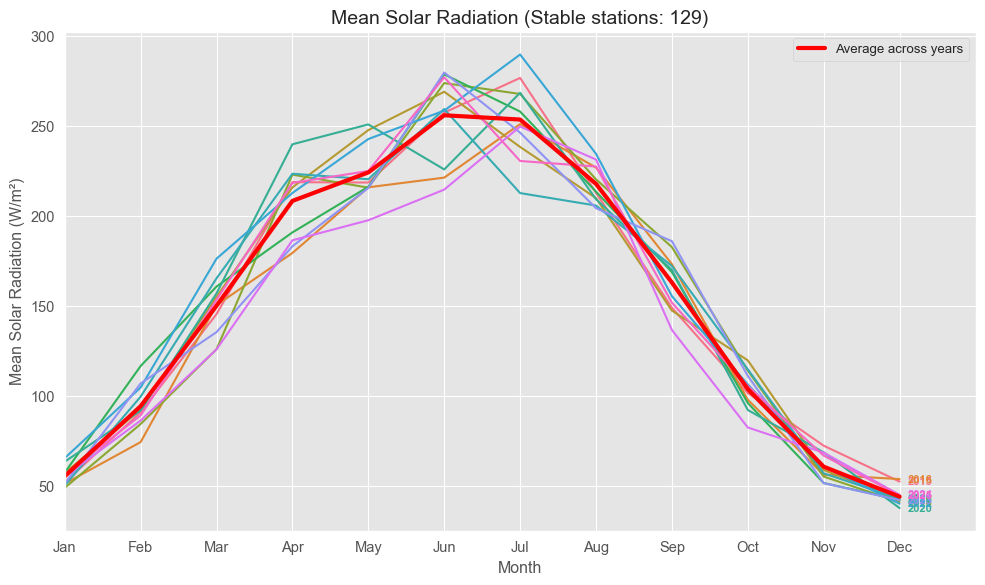
\includegraphics[width=\linewidth]{figures_and_tables/mean_wind_2015_2025.png}
        %\caption{Première image}
    \end{minipage}\hfill
    \begin{minipage}{0.48\textwidth}
        \centering
        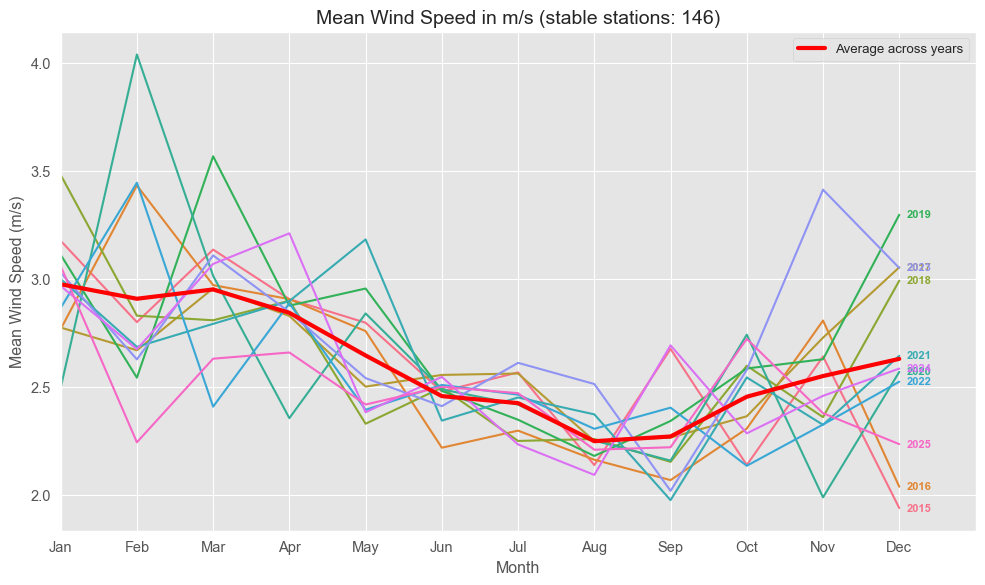
\includegraphics[width=\linewidth]{figures_and_tables/mean_solar_2015_2025.png}
        %\caption{Deuxième image}
    \end{minipage}
    %\caption{Mean wind speed and solar radiation from 2015 to 2025.}
    % --- suggestion ---
    \caption{Mean wind speed (left) and mean solar radiation (right), 2015--2025.}
    % Note : préciser aussi la fréquence temporelle et le mode d'agrégation entre stations si ces informations ne figurent pas déjà sur les graphiques.
    \label{fig:fig_lubin}
\end{figure}


% ## Results we are looking for
% - explain that we will use the data to determine complementarity though data description and correlation analysis. 

% We aim here at studying the complementarity between wind speed and solar radiation to account for a potential electricity production complementarity between wind turbines and PVs. We will use correlations criteria as used by \citet{Canales2019} and product descriptive statistics allowing us to analyse such complementarity. These statistics will cover a seasonal analysis, data stratification accounting for elevation and geographic zone using daily and monthly data.
% --- suggestion ---
We aim to assess complementarity between wind and solar resources and its potential implications for electricity generation. Following \citet{Canales2019}, we will use correlation measures, complemented by descriptive statistics. Using daily and monthly data, we will examine seasonal patterns and compare complementarity across elevation classes and geographical areas.
% Note : « correlation measures » remplace « correlations criteria » ; « complemented by descriptive statistics » corrige « product descriptive statistics ». « Elevation bands » suppose un regroupement par classes d'altitude ; adapter si l'altitude est traitée autrement.

\bibliographystyle{plainnat}
\bibliography{resources}

\end{document}
